% CS224R Project Milestone Report
\documentclass{article}

\usepackage[preprint,nonatbib]{cs224r_2026}
\usepackage[utf8]{inputenc}
\usepackage[T1]{fontenc}
\usepackage[colorlinks=true,linkcolor=blue,citecolor=blue,urlcolor=blue]{hyperref}
\usepackage{url}
\usepackage{booktabs}
\usepackage{amsfonts}
\usepackage{nicefrac}
\usepackage{microtype}
\usepackage{xcolor}
\usepackage{amsmath}
\usepackage{graphicx}
\usepackage{pgfplots}
\pgfplotsset{compat=1.18}
\usepackage{fancyhdr}
\usepackage{caption}
\usepackage{multicol}

% Tight spacing
\usepackage{enumitem}
\setlist{nosep,leftmargin=*}
\usepackage{titlesec}
\titlespacing*{\section}{0pt}{0.6ex plus 0.2ex minus 0.2ex}{0.2ex plus 0.1ex}

% Compact captions
\captionsetup{font=small,skip=2pt}

\pagestyle{fancy}
\fancyhf{}
\fancyhead[C]{CS224R Project Milestone}
\renewcommand{\headrulewidth}{0.4pt}

\renewcommand{\maketitle}{
  \begin{center}
    {\bf \large Enhancing SINGER: Onboard Visual Drone Navigation through Iterative Imitation Learning and Reinforcement Fine-Tuning}\\
    \vspace{0.05cm}
    {\bf Team Members:} Erwin Poussi \quad {\bf Email:} erwinpi@stanford.edu\\
    \vspace{0.1cm}
  \end{center}
}

\begin{document}

\maketitle
\vspace{-0.3cm}

\begin{multicols}{2}

\section{Problem Overview}

SINGER~[1] is a language-conditioned onboard visual navigation policy for drones, developed at the Stanford Multi-Robot Systems Lab where I work. The drone navigates autonomously using only onboard RGB frames, avoiding obstacles to reach a target object specified by a natural language query, within a photorealistic 3D Gaussian Splatting simulation~[2]. At the time of the proposal, the baseline behavioral cloning (BC) policy trained on expert RRT trajectories achieved roughly 80\% success rate after we engineered some visually inferred goal-relative bearing and elevation with respect to the drone camera as additional input for the policy. The goal remains to push toward 100\% success for safe, fully autonomous drone navigation.

\section{Experiments}

Our main experimental effort since the proposal has been on two fronts, namely iterative DAgger for distribution shift and action chunking for long-horizon prediction.

\textbf{Iterative DAgger.}
As proposed, we implemented iterative DAgger~[3] within the SINGER pipeline. This choice was motivated by the fact that we were observing strong distributional shift between the learned policy and the expert, resulting in critical compounding errors that would cause the model to collide. To mitigate this, after a BC pretraining over 210 trajectories, we sample 24 trajectories per iteration randomly and deploy the learned pilot in simulation, letting it navigate on its own. At every visited state, we record the action the expert would have taken at that same state, where the expert is an MPC controller tracking a reference RRT trajectory. This effectively relabels the pilot's on-policy trajectory with expert corrections, exposing the learner to its own mistakes while providing the correct recovery actions. We then retrain the policy on these aggregated relabeled demonstrations, progressively closing the gap between the states seen during training and those encountered during deployment. Over 11 iterations, the policy steadily improved and peaked at iteration~8 with 92\% success over 50 training flights for 3 different objects before starting to degrade (Figure~\ref{fig:dagger_curve}). The final benchmark confirmed \textbf{88.0\% success} and \textbf{8.0\% collision} on unseen testing flights different from the training ones, a +51.3pp end-to-end improvement over the original pre-centroid BC baseline. We are quite satisfied with these results as they meet good performance.

\begin{center}
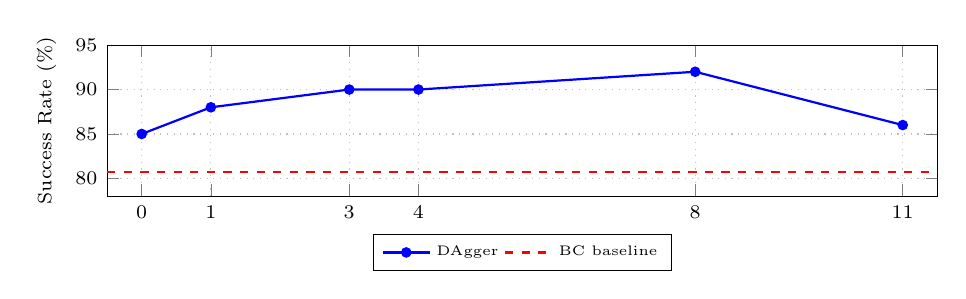
\begin{tikzpicture}
\begin{axis}[
    width=\columnwidth, height=3.5cm,
    xlabel={DAgger Iteration}, ylabel={Success Rate (\%)},
    xmin=-0.5, xmax=11.5, ymin=78, ymax=95,
    xtick={0,1,3,4,8,11},
    ytick={80,85,90,95},
    grid=major, grid style={dotted,gray!50},
    mark size=1.5pt,
    tick label style={font=\scriptsize},
    label style={font=\scriptsize},
    legend style={font=\tiny, at={(0.5,-0.25)}, anchor=north, legend columns=2},
]
\addplot[blue, thick, mark=*] coordinates {
    (0,85) (1,88) (3,90) (4,90) (8,92) (11,86)
};
\addplot[red, dashed, thick, domain=-0.5:11.5] {80.7};
\legend{DAgger, BC baseline}
\end{axis}
\end{tikzpicture}
\captionof{figure}{DAgger success rate across iterations, peaking at iter~8 (92\%) before degrading.}
\label{fig:dagger_curve}
\end{center}

\textbf{Action chunking and flow matching.}
Beyond DAgger, we explored whether predicting further into the future could help. Inspired by DreamZero~[4] and the course material, we trained SINGER with action chunking ($H{=}10$ future actions). However, BC success dropped to roughly 70\% (from 80\%), so we did not pursue DAgger on this variant. We attribute this to the ``blindness'' of our RRT expert, which plans geometric paths without visual feedback and sometimes produces sinuous trajectories with unnecessary detours (Figure~\ref{fig:sinuous}). When BC imitates these inconsistent future actions, the policy receives contradictory supervision, for instance learning ``go left'' when the target is on the right. Action chunking amplifies this since a longer horizon compounds the expert's non-visual inconsistencies. We also tried flow matching to handle multimodal demonstrations, but DAgger remained the most effective approach.

\begin{center}
\includegraphics[width=\columnwidth]{expert_sinuous_traj.png}
\captionof{figure}{RRT reference trajectory (blue) toward the clock (left), where the expert tries to MPC-track it (red) but makes sinuous detours and actually collides in this case, illustrating that our expert is far from ideal.}
\label{fig:sinuous}
\end{center}

\section{Research Hypothesis and Future Steps}

Given these results, our main direction, iterative DAgger combined with our feature engineering, has proven effective (+51.3pp end-to-end compared to vanilla SINGER training) and we are not deviating from the original plan. The DreamZero-inspired long-horizon action prediction and world modeling directions that we proposed will be left for further study, once we obtain a better expert and a more reliable target detection pipeline, since action chunking proved detrimental in our current setting due to the blindness of our expert. We therefore continue to focus on single-step prediction. We investigated failure modes when SINGER is deployed and it points to input quality (false positive goal detections that make the policy drift toward wrong objects) and expert data quality (sinuous paths as illustrated in Figure~\ref{fig:sinuous}) as the main bottlenecks rather than the learning algorithm itself. Since we synthesize all our data in 3D Gaussian Splatting simulation, generating high-quality expert demonstrations is computationally expensive and the full BC-to-DAgger pipeline takes roughly two days end-to-end, which makes online RL exploration prohibitively costly and motivates offline RL instead.

Concretely, we plan to pursue the following directions.

\textbf{Within the scope of RL for this class}, we realistically plan to accomplish at least the following.
\begin{itemize}
\item \textbf{Offline RL fine-tuning} notably using Advantage Weighted Regression (AWR) to help SINGER discriminate good from bad expert demonstrations and hopefully bridge the remaining performance gap on identified failure modes. Ideally we would generate multiple trajectories per starting position for all training flights so the algorithm can compare different paths toward the same goal, but since this linearly increases compute time we will focus on doing so on failure trajectories for targeted improvement and fine-tuning, which is more computationally feasible as we have few failed trajectories that represent extreme cases.
\end{itemize}

\textbf{Beyond RL}, some engineering choices we believe are critical to help the model learn better, and that we consider pursuing for further SINGER development.
\begin{itemize}
\item \textbf{Improved perception} since we are doing purely visual navigation and our current target detection model produces several false positives that induce the policy into error, making it drift toward objects it thinks are the target but are not, which we do not count as a success in our metrics.
\item \textbf{Depth estimation} via CARE~[5] to help reduce collisions by giving the model an idea of depth, voids, and imminent obstacles.
\item \textbf{Long-horizon planning} once we have sorted the expert blindness problem, we will consider action chunking as in DreamZero and also target-out-of-sight dynamics estimation, but this requires first having reliable target detection and semantic perception.
\end{itemize}

\section{Team Contributions}

I, Erwin Poussi, am the sole contributor of this project.

\end{multicols}

\vspace{-0.1cm}
\noindent\rule{\textwidth}{0.4pt}
{\footnotesize\noindent [1]~Adang et al., \textit{SINGER}, arXiv:2509.18610, 2025.\;
[2]~Low et al., \textit{SOUS VIDE}, arXiv:2412.16346, 2024.\;
[3]~Ross et al., \textit{DAgger}, AISTATS, 2011.\;
[4]~Ye et al., \textit{DreamZero}, arXiv:2602.15922, 2026.\;
[5]~Kim et al., \textit{CARE}, arXiv:2506.03834, 2025.}

\end{document}
